\section{Results and evaluation} \label{sec:results}

\subsection{Overview of datasets used for testing}

A couple of different datasets will be used for testing and evaluating the
implementation of the distance metrics and clustering algorithms presented in
section \ref{sec:methods}. These datasets will be briefly presented in this
section.

\begin{description}
  \item[\texttt{SILVA}] \hfill \\
    The dataset \texttt{SILVA\_119\_SSURef\_tax\_silva.fasta} has a size of
    around 2.3GB and contains $1,583,830$ RNA sequences.

  \item[\texttt{RDP}] \hfill \\
    The dataset \texttt{RDP\_Pro\_Full.sort.fna} has a size of around 3.5 GB
    and contains $3,019,928$ DNA sequences.
\end{description}

Various statistics about the datasets are shown in figure \ref{fig:data_stats}.
The error ratio is the ratio between the number of non DNA/RNA bases, i.e. 'R',
'Y', 'K' etc., and the total number of characters in the sequences.

\begin{figure}[H]
  \centering
  \begin{tabular}{c |  c | c | c | c | c}
    Dataset        & Avg. len. & Min. len. & Max. len. & Median len. & Error ratio \\
    \hline
    \texttt{SILVA} & 1,415.46  & 900       & 3,845     & 1,389       & 0.000156146 \\
    \texttt{RDP}   & 1,044.19  & 400       & 2,922     & 1,132       & 0.000798764 \\
  \end{tabular}
  \caption{Various information about the different datasets.}
  \label{fig:data_stats}
\end{figure}

% SILVA:
% avg_len:       1415.46
% min_len:       900
% max_len:       3845
% median:        1389
% dirty:         350055
% dirty/sum_len: 0.000156146

% RDP:
% avg_len:       1044.19
% min_len:       400
% max_len:       2922
% median:        1132
% dirty:         2518801
% dirty/sum_len: 0.000798764


\subsection{Testing the distance metric on altered sequences}
\label{sec:altered_sequences}
%TODO: Misleading title?

% TODO: can't get this crap right....
%A few different sets of highly similar sequences were synthetically constructed
%from real data and used in the evaluation the distance metric.
%
%A sequence was randomly chosen from \texttt{SILVA} and four sets, each
%containing ten copies of this sequence, were made. For each sequence in the
%first two sets, a list of random indices in the sequence was generated and in
%each of these indices in the sequence, a substitution for a different, randomly
%chosen nucleotide was made. For the first set, this list was of legnt

Two different sets of highly similar sequences was constructed from a real
world sequence from \texttt{SILVA} and this was used in the evaluation of the
distance metric.

One sequence was chosen, 10 copies of this sequences were made and to each of
these copies, a few alterations were made. In the first set, a list of random
indices in the sequence were generated and in each of these indices in the
sequence, a substitution for a different, randomly chosen nucleotide was made.
This was done twice, for different degrees of alteration, and the number of
alterations was equal to respectively 1\% and 2\% of the length of the
sequence.

In the second set, the same number of alterations to individual nucleotides
were made, but in this case they were grouped into alterations of substrings of
length 5 (one such group being of length less than 5 if the number of
alterations were not a multiple of 5).

For illustration, figure \ref{fig:alterations} shows an original sequence in
the first line, the single edits alterated sequence in the second line and the
chunk alterated sequence in the third line.

\newcommand{\tc}[1]{\textcolor{red}{#1}}
\begin{figure}[H]
  \centering
  \texttt{AAAAAAAAAAAAAAAAAAAAAA} \\
  \texttt{AAAAA\tc{T}AA\tc{C}AAAA\tc{G}AAAA\tc{T}AAA} \\
  \texttt{AAA\tc{TC}AAAAAAAAAA\tc{GG}AAAAA}
  \caption{Two types of alterations to sequences: the original sequence in the
    first line, single edit alterations in the second line and chunks of edits
    in the third line.}
  \label{fig:alterations}
\end{figure}

The $k$-mer based distance metric, presented in section
\ref{sec:kmer_distance}, is expected to be more sensitive to a number of
individual changes than to the same number of changes made in chunks. This test
serves to confirm this expectation and to give an insight into the change in
$k$-mer distance when performing a controlled number of edits.

The similarities between the original sequence from \texttt{SILVA} and the 10
altered sequences, for the four different types of alterations, are shown in
figure \ref{fig:altered_seqs_similarities}.

\begin{figure}[H]
  \centering
  \begin{tabular}{c|c||c|c}
    \multicolumn{2}{c||}{single edits}  & \multicolumn{2}{c}{chunk edits} \\
    \hline\hline
    1\%   &   2\%                   &   1\%   &   2\% \\
    \hline
    0.944   & 0.889                     & 0.980     & 0.960 \\
    0.947   & 0.887                     & 0.979     & 0.960 \\
    0.944   & 0.893                     & 0.979     & 0.960 \\
    0.941   & 0.902                     & 0.979     & 0.961 \\
    0.944   & 0.894                     & 0.979     & 0.958 \\
    0.947   & 0.894                     & 0.979     & 0.958 \\
    0.941   & 0.895                     & 0.982     & 0.958 \\
    0.945   & 0.891                     & 0.979     & 0.961 \\
    0.945   & 0.889                     & 0.979     & 0.958 \\
    0.946   & 0.897                     & 0.981     & 0.958
  \end{tabular}
  \caption{Similarity measures for 1\% and 2\% single edits, respectively,
    and 1\% and 2\% chunk edits, respectively, to 10 copies of a single
    sequence.}
  \label{fig:altered_seqs_similarities}
\end{figure}

As expected, the single edits result in a lower similarity that the
corresponding chunk edits. This is because five individual changes will affect
the count of up to $5 \cdot k$ $k$-mers, while five changes in sequence will
only affect up to $4+k$ $k$-mers.


\subsection{Evaluating \textsc{K-Clust} on a synthetic dataset}
\label{sec:synth_dataset}

A synthetic dataset was constructed for evaluating the algorithm
\textsc{K-Clust}'s ability to find the right clusters in a dataset with a
clearly correct, expected clustering output.

A set of 380 sequences with mutual similarities of at most 0.6 was extracted
from \texttt{SILVA}, using the \textsc{K-Dist} distance metric (algorithm
\ref{alg:K-Dist}) with parameter $k=5$. For each of these sequences, 999 copies
were made and chunks of changes were made to these as described above in
section \ref{sec:altered_sequences}, corresponding to 2\% of the characters of
each sequence. This yields a set of $380,000$ sequences with 380 expected
clusters, which each should contain sequences with similarities of
approximately $0.92$ since all sequences are changed and a 2\% change to a
sequence gives an average similarity from the original sequence of around
$0.96$, cf. section \ref{sec:altered_sequences}.

The sequences expected to be in the same cluster was given the same description
in the \texttt{FASTA} file, i.e. the same text string after ``>'', to make it
easy to evaluate the result from the clustering.

The synthetic dataset was made fairly large, both in number of sequences and in
number of expected clusters, to be able to properly test the clustering
algorithm's ability to search for the correct centroid and not stop the search
prematurely which would result in a new cluster being created and a different
clustering result than the expected one.

As hoped, running \texttt{klust} on the constructed dataset gives a clustering
output consisting of 380 clusters with 1000 sequences in each (including the
centroid). The terminal output from the program is shown in figure
\ref{fig:synth_silva_output} in appendix \ref{app:synth_dataset} and an excerpt
from the clustering ouput file created by the program is shown in figure
\ref{fig:synth_silva_clustering} in the same appendix.


\subsubsection{Multidimensional scaling of the synthetic dataset}

Multidimensional scaling (MDS) of the distance matrix of the sequences in the
synthetic dataset was made and the sequences in the same cluster from the above
test were colored with the same color and the centroid with a ``+'' marker.

The MDS of the first 400 sequences of the synthetic dataset, i.e. the first 40
clusters, is shown in figure \ref{fig:mds_synth}.

\begin{figure}[H]
  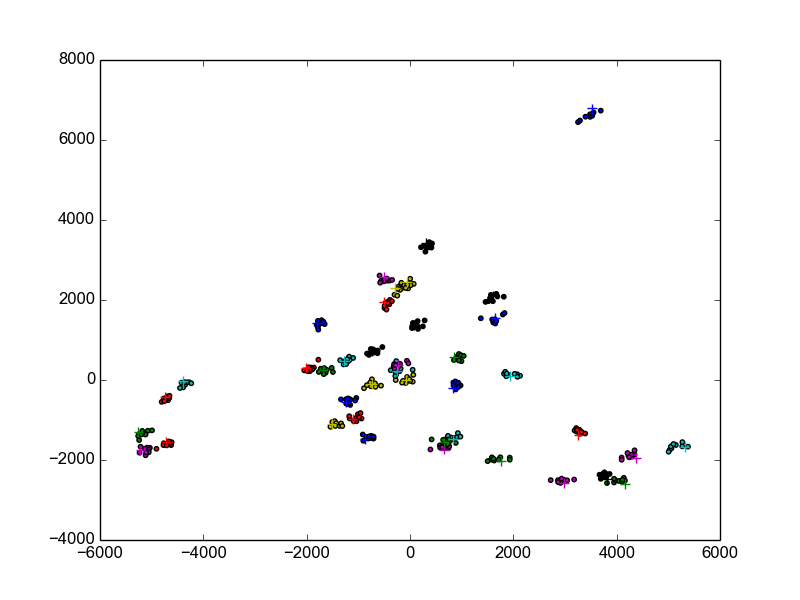
\includegraphics[width=\textwidth]{graphics/MDS_t-SNE_synth_silva_400.png}
  \caption{Multidimensional scaling of the first 400 sequences (40 clusters) of
    the synthetic dataset.}
  \label{fig:mds_synth}
\end{figure}




\subsection{Evaluating distance metric}

To evaluate the \textsc{K-Dist} algorithm, presented in section
\ref{sec:kmer_distance}, the Levenshtein distance was used as reference. Since
the Levenshtein distance does not produce values between $0$ and $1$, the
Jaccard index was used here as well. %TODO: How is it used

In figure \ref{fig:Levenshtein_vs_Kmer} are three scatter plots with the
Levenshtein distance on the $y$-axis and the distance that \textsc{K-Dist}
produces on the $x$-axis. The three plots are with $k=4, k=6$ and $k=8$ respectively.

The scatter plots gives an indication about when and how sensitive our
implemented distance metric is.

When $k=4$, there is a linear relation when the identity $I>0.9$, but when
$I<0.9$ there is too much variance to express it as a linear function.

With $k=6$, there seems to be a linear relation when $I>0.8$. When $I<0.8$ there
is more variance, though less than when $k=4$.

When $k=8$, it is very similar to $k=6$. It seems there is a linear relation
for $I>0.8$ again and when $I<0.8$ the variance is greater.
%TODO: This section is shit

\begin{figure}[H]
  \begin{subfigure}[b]{0.5\textwidth}
    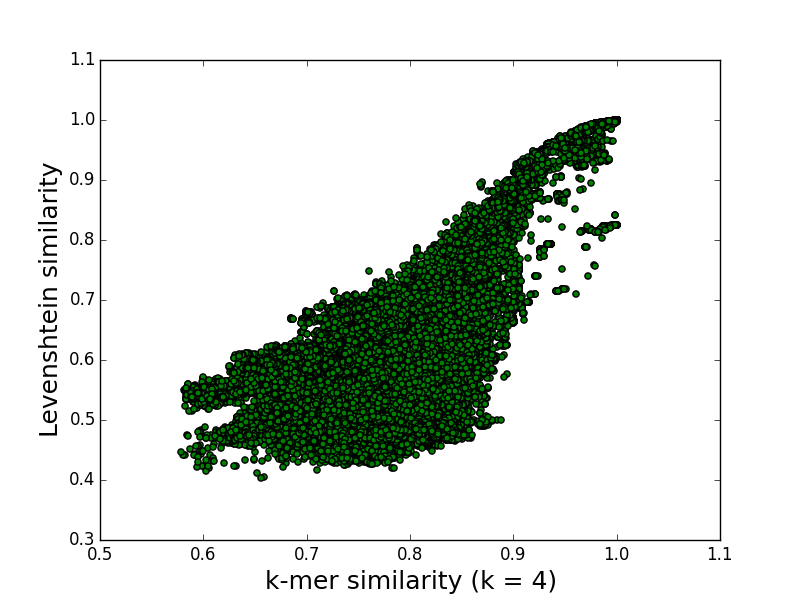
\includegraphics[scale=0.34]{graphics/k4.png}
  \end{subfigure}
  \begin{subfigure}[b]{0.5\textwidth}
    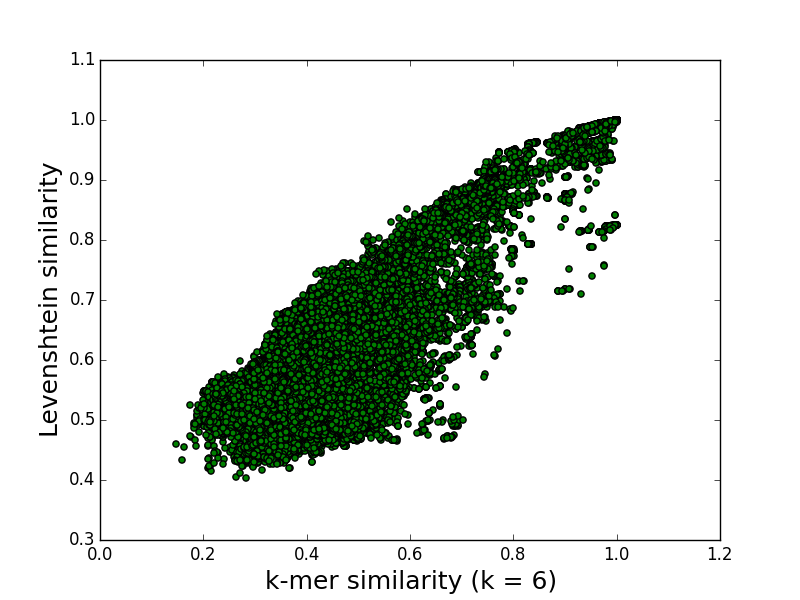
\includegraphics[scale=0.34]{graphics/k6.png}
  \end{subfigure}

  \centering
  \begin{subfigure}[b]{0.5\textwidth}
    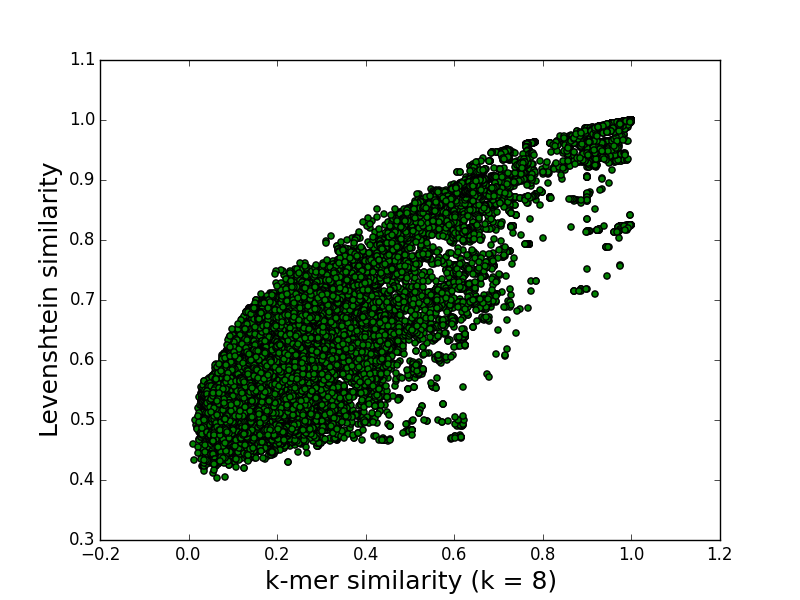
\includegraphics[scale=0.34]{graphics/k8.png}
  \end{subfigure}
  \caption{Comparison of Levenshtein distance and our implementation of the
  $k$-mer distance using windows and Jaccard index.}
  \label{fig:Levenshtein_vs_Kmer}
\end{figure}

\subsection{Evaluating clustering algorithm on real data}

This section describes different ways of evaluating the \textsc{K-Clust}
algorithm on real \texttt{RNA} data (\texttt{SILVA}) using multidimensional
scaling (MDS) and t-distributed Stochastic Neighbor Embedding (t-SNE). This was
done using \texttt{Python} with \texttt{matplotlib} and \texttt{scikit-learn}.

One example of this multidimesional scaling on the distance matrix for the
first 500 sequences of \texttt{SILVA} is shown in figure \ref{fig:mds_tsne}.
The centroids found using the clustering algorithm \textsc{K-Clust}, with
similarity threshold 0.85, $max\_rejects$ 8 and $k$ 6, are pinpointed in the
plot and labeled with the numbers of the sequences in the order they were read.

\begin{figure}[h!]
  \centering
  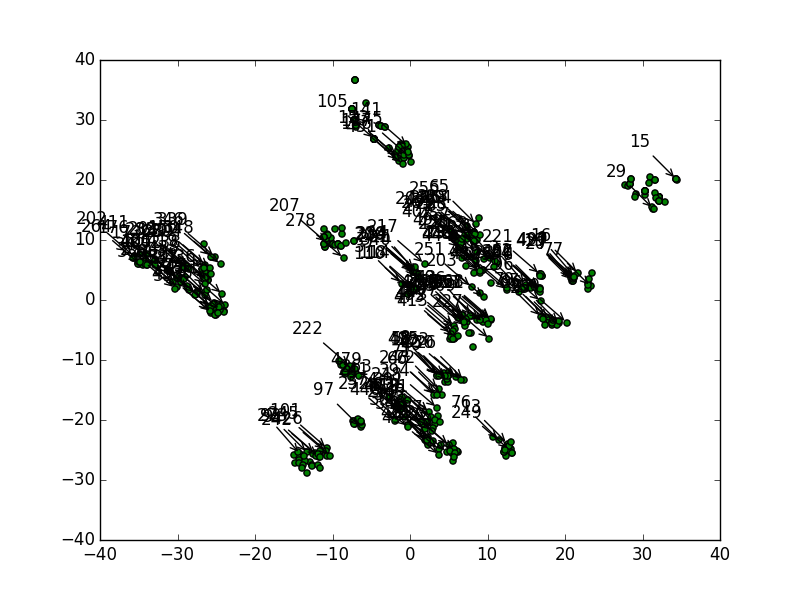
\includegraphics[width=\textwidth]{graphics/MDS_t-SNE_SILVA_500.png}
  \caption{Multidimensional scaling with annotations on centroids.}
  \label{fig:mds_tsne}
\end{figure}

Another test is what parameters and settings works well for the performance of
the program and quality of the clustering. The table in
\ref{app:klust_data_parameters} shows output data from running the first
$100,000$ sequences from \texttt{SILVA} with different parameters. Sorting by
increasing length is on average $21.65\%$ faster and never slower than not
sorting. It is also on average $42.63\%$ faster and never slower than sorting
by decreasing length. Furthermore, sorting by increasing length on average has
$8.77\%$ fewer clusters and never more clusters than not sorting. It has
$25.07\%$ fewer clusters on average and never more clusters than when sorting
by decreasing length. \\
So it shows that sorting by increasing length is always preferrable, so in the following tests this will be used.

\subsection{Results}
\begin{figure}[H]
  \centering
  \begin{tabular}{ c | c }
    Metric                                        & Comparisons/second      \\
    \hline \hline
    Dynamic programming (bottom up) Levenshtein   & $\sim$ 70               \\
    \hline
    d2-distance with window, $k=4$                & $\sim$ 73000            \\
    \hline
    d2-distance with window, $k=6$                & $\sim$ 63000            \\
    \hline
    d2-distance with window, $k=8$                & $\sim$ 24000            \\
  \end{tabular}
  \caption{Performance of different distance metrics.}
\end{figure}

\begin{figure}[H]
  \centering
  \begin{tabular}{ p{12em} | c | c }
    Method  & Throughput/second   & \# of clusters \\
    \hline \hline
    \textsc{Simple-Clust}, $k=4$,
    $max\_rejects=8$, $id=0.97$     & $\sim$ 11,400  & 444,654  \\
    \hline
    \textsc{Simple-Clust}, $k=5$,
    $max\_rejects=8$, $id=0.97$     & $\sim$ 10,700  & 461,266  \\
    \hline
    \textsc{Simple-Clust}, $k=6$,
    $max\_rejects=8$, $id=0.97$     & $\sim$ 9,575   & 470,516  \\
    \hline
    \textsc{Simple-Clust}, $k=7$,
    $max\_rejects=8$, $id=0.97$     & $\sim$ 6,350   & 474,463  \\
    \hline
    \textsc{Simple-Clust}, $k=8$,
    $max\_rejects=8$, $id=0.97$     & $\sim$ 2,750   & 475,465  \\
  \end{tabular}
  \caption{Performance of different clustering methods and different $k$-mer
  sizes. Sequence data:
           \texttt{RDP\_Pro\_Full\_sort.fna}. Count: 500,000. Throughput
           specifies the number of sequences clustered per second (including
           results output to file), but excludes reading the input file.}
\end{figure}

Results of performance

\begingroup
\setlength{\LTleft}{-20cm plus -1fill}
\setlength{\LTright}{\LTleft}
\begin{longtable}{c|cc|c|c|c|c}
  \multirow{2}{*}{}
  Clustering & \multicolumn{2}{c|}{Parameters} & Sorting & Time & Throughput & Max memory \\
  algorithm & & & & (sec.) & (seqs./sec.) & \\
  \hline \hline
  \multirow{3}{*}
  {\textsc{K-Clust}} & k & 5 & & & & \\
                     & id & 0.8 & no & 623.622 & 2539.73 & 1013 MB \\
                     & m & 8 & & & & \\
  \hline
  \multirow{3}{*}
  {\textsc{K-Clust}} & k & 5 & & & & \\
                     & id & 0.8 & incr. & 501.697 & 3156.94 & 1013 MB \\
                     & m & 8 & & & & \\
  \hline
  \multirow{3}{*}
  {\textsc{K-Clust}} & k & 5 & & & & \\
                     & id & 0.85 & no & 1314.18 & 1205.18 & 1013 MB \\
                     & m & 8 & & & & \\
  \hline
  \multirow{3}{*}
  {\textsc{K-Clust}} & k & 5 & & & & \\
                     & id & 0.85 & incr & 1144.55 & 1383.81 & 1013 MB \\
                     & m & 8 & & & & \\
  \hline
  \multirow{3}{*}
  {\textsc{K-Clust}} & k & 5 & & & & \\
                     & id & 0.90 & no & 2982.8 & 530.988 & 1030 MB \\
                     & m & 8 & & & & \\
  \hline
  \multirow{3}{*}
  {\textsc{K-Clust}} & k & 5 & & & & \\
                     & id & 0.90 & incr. & 2578.88 & 614.155 & 1021 MB \\
                     & m & 8 & & & & \\
  \hline
  \multirow{3}{*}
  {\textsc{K-Clust}} & k & 6 & & & & \\
                     & id & 0.8 & no & 1021.26 & 1550.86 & 1014 MB \\
                     & m & 8 & & & & \\
  \hline
  \multirow{3}{*}
  {\textsc{K-Clust}} & k & 6 & & & & \\
                     & id & 0.8 & incr. & 856.785 & 1848.57 & 1014 MB \\
                     & m & 8 & & & & \\
  \hline
  \multirow{3}{*}
  {\textsc{K-Clust}} & k & 6 & & & & \\
                     & id & 0.85 & no & 2014.1 & 786.373 & 1014 MB \\
                     & m & 8 & & & & \\
  \hline
  \multirow{3}{*}
  {\textsc{K-Clust}} & k & 6 & & & & \\
                     & id & 0.85 & incr. & 1812.02 & 874.066 & 1012 MB \\
                     & m & 8 & & & & \\
  \hline
  \multirow{3}{*}
  {\textsc{K-Clust}} & k & 6 & & & & \\
                     & id & 0.9 & no & 4245.53 & 373.059 & 1045 MB \\
                     & m & 8 & & & & \\
  \hline
  \multirow{3}{*}
  {\textsc{K-Clust}} & k & 6 & & & & \\
                     & id & 0.9 & incr. & 3450.59 & 459.003 & 1039 MB \\
                     & m & 8 & & & & \\
  \\
  \caption{Performance results for different parameters of
    \texttt{klust} on the entire \texttt{SILVA} dataset.}
  \label{fig:full_silva_results_performance}
\end{longtable}
\endgroup

Results of the clustering.

\begingroup
\setlength{\LTleft}{-20cm plus -1fill}
\setlength{\LTright}{\LTleft}
\begin{longtable}{c|cc|c|c|cc}
  Clustering algorithm & \multicolumn{2}{c|}{Parameters} & Sorting & Clusters & \multicolumn{2}{c}{Cluster sizes} \\
  & & & & & \\
  \hline \hline
  \multirow{3}{*}
  {\textsc{K-Clust}} & k & 5 & & & Max & 68542 \\
                     & id & 0.8 & no & 70080 & Avg & 22.6003 \\
                     & m & 8 & & & Min & 1 \\
  \hline
  \multirow{3}{*}
  {\textsc{K-Clust}} & k & 5 & & & Max & 57121 \\
                     & id & 0.8 & incr. & 60111 & Avg & 26.3484 \\
                     & m & 8 & & & Min & 1 \\
  \hline
  \multirow{3}{*}
  {\textsc{K-Clust}} & k & 5 & & & Max & 76164 \\
                     & id & 0.85 & no & 112063 & Avg & 14.1334 \\
                     & m & 8 & & & Min & 1 \\
  \hline
  \multirow{3}{*}
  {\textsc{K-Clust}} & k & 5 & & & Max & 57885 \\
                     & id & 0.85 & incr. & 98354 & Avg & 16.1034 \\
                     & m & 8 & & & Min & 1 \\
  \hline
  \multirow{3}{*}
  {\textsc{K-Clust}} & k & 5 & & & Max & 46915 \\
                     & id & 0.9 & no & 179222 & Avg & 8.83725 \\
                     & m & 8 & & & Min & 1 \\
  \hline
  \multirow{3}{*}
  {\textsc{K-Clust}} & k & 5 & & & Max & 71407 \\
                     & id & 0.9 & incr. & 159812 & Avg & 9.91058 \\
                     & m & 8 & & & Min & 1 \\
  \hline
  \multirow{3}{*}
  {\textsc{K-Clust}} & k & 6 & & & Max & 87170 \\
                     & id & 0.8 & no & 93055 & Avg & 17.0204 \\
                     & m & 8 & & & Min & 1 \\
  \hline
  \multirow{3}{*}
  {\textsc{K-Clust}} & k & 6 & & & Max & 60256 \\
                     & id & 0.8 & incr. & 86905 & Avg & 18.2248 \\
                     & m & 8 & & & Min & 1 \\
  \hline
  \multirow{3}{*}
  {\textsc{K-Clust}} & k & 6 & & & Max & 63452 \\
                     & id & 0.85 & no & 138023 & Avg & 11.4751 \\
                     & m & 8 & & & Min & 1 \\
  \hline
  \multirow{3}{*}
  {\textsc{K-Clust}} & k & 6 & & & Max & 79599 \\
                     & id & 0.85 & incr. & 127711 & Avg & 12.4017 \\
                     & m & 8 & & & Min & 1 \\
  \hline
  \multirow{3}{*}
  {\textsc{K-Clust}} & k & 6 & & & Max & 43381 \\
                     & id & 0.9 & no & 207890 & Avg & 7.6186 \\
                     & m & 8 & & & Min & 1 \\
  \hline
  \multirow{3}{*}
  {\textsc{K-Clust}} & k & 6 & & & Max & 49479 \\
                     & id & 0.9 & incr. & 191361 & Avg & 8.27666 \\
                     & m & 8 & & & Min & 1 \\
  \\
  \caption{Clustering results for different parameters of
    \texttt{klust} on the entire \texttt{SILVA} dataset.}
  \label{fig:full_silva_results_clusters}
\end{longtable}
\endgroup

\subsection{Comparing with UCLUST on real life data}
% Testing USEARCH 32-bit on real data
% Testing clustering algorithm with d2 distance and comparing performance to
% USEARCH.
Running \texttt{USEARCH} on the file
\texttt{SILVA\_119\_SSURef\_tax\_silva.fasta} after it is sorted with
parameters \texttt{-clust\_smallmem} and \texttt{-id 0.95} produces the
following output

\begin{figure}[H]
\begin{lstlisting}[style=output-style]
28:39 1.1Gb  100.0\% 117205 clusters, max size 83904, avg 13.5
      Seqs  1583830 (1.6M)
  Clusters  117205 (117.2k)
  Max size  83904 (83.9k)
  Avg size  13.5
  Min size  1
Singletons  67410 (67.4k), 4.3\% of seqs, 57.5\% of clusters
   Max mem  1.1Gb
      Time  28:41
Throughput  920.3 seqs/sec.
\end{lstlisting}
  \caption{Output from \texttt{USEARCH} clustering.}
  \label{fig:uclust_silva}
\end{figure}

Benchmarks from \textsc{K-Clust} can be seen in the previous section.
% Running our implementation of the same file but unsorted and with
% \texttt{id=0.9, k=6} og \texttt{max\_rejects=8} produces the following

% \begin{figure}[H]
% \begin{lstlisting}[style=output-style]
% Reading 1583830 sequences...
% Finished reading:
% Time: 24.8109 sec.
% Seqs/sec: 63836
% Clustering 1583830 sequences...
% 26.4602
% # of clusters: 1364006
% Finished clustering:
% Time: 187.355 sec.
% Throughput: 8453.63seqs/sec.
% \end{lstlisting}
% %TODO caption and label?
% \end{figure}

% Even though the \texttt{id}'s do not represent the same threshold due to it
% being two different distance metrics we do get a lot more clusters. Running
% it with similar \texttt{id}'s produces almost the same amount of clusters, so
% the problem lies in the way we choose our centroids we compare a query
% sequence with.

% Our implementation, however, is faster by a factor of $10$. This can be
% attributed to our choice of distance metric.

%TODO: This section is also chaos
%Possibly things to look into: confusion matrix, Rand index, normalized
%mutual information (article: Comparing Clusterings - An Overview).

%TODO: Yeah well, results not done - update tables with other algorithms etc.
